\chapter{Implementacja}
W niniejszym rozdziale przedstawiona zostanie szczegółowa analiza aspektów technicznych związanych z implementacją aplikacji. Na początku zaprezentowane zostaną wykorzystane narzędzia wraz z uzasadnieniem ich wyboru w kontekście wymagań projektowych. Następnie omówiona zostanie architektura warstw systemu oraz komunikacja między nimi. W dalszej części rozdziału szczegółowo opisane zostaną poszczególne moduły systemu oraz ich wzajemne powiązania. Ostatnia część poświęcona będzie omówieniu implementacji kluczowych funkcjonalności: mechanizmu publikacji ogłoszeń, modułu wizualizacji tras na mapie oraz algorytmu rekomendacji ogłoszeń.

\section{Opis narzędzi}
Aplikacja została wykonana w technologii webowej, przy użyciu fullstackowego frameworka \texttt{Next.js} \cite{Next} (w wersji \texttt{15.1.3}). Jest to popularny sposób tworzenia aplikacji webowych, zapewniający wiele przydatnych funkcji poprawiających optymalizacje. Między innymi \texttt{Next.js} skraca czas potrzebny do załadowania aplikacji poprzez renderowanie kodu \texttt{HTML} strony, już podczas kompilacji aplikacji. Został on oparty na innym frameworku - React \cite{React}, jest to jedna z najpopularniejszych bibliotek \texttt{JavaScript} do budowania interfejsów użytkownika. Opiera się on na koncepcji komponentów - niezależnych, wielokrotnego użytku bloków interfejsu. Komponenty te w  \texttt{Next.js} są renderowane po stronie serwera, co znacząco przyspiesza pierwsze ładowanie strony. Dodatkowo renderowanie komponentów aplikacji po stronie serwera, pozytywnie wpływa na algorytmy \texttt{SEO}, co skutkuje lepszym pozycjonowaniem serwisu w wyszukiwarkach internetowych. \texttt{Next.js} posiada zintegrowane rozwiązanie fullstackowe, oznacza to, że zarówno backend jak i frontend aplikacji wykorzystują tę samą bazę kodu. Takie podejście znacząco upraszcza proces developmentu i utrzymania aplikacji, eliminując potrzebę zarządzania oddzielnymi projektami dla części serwerowej i klienckiej. Dodatkowo ułatwia proces wdrożenia aplikacji na środowisko produkcyjne.

Zamiast standardowych klas \texttt{CSS}, do interfejsu użytkownika została użyta biblioteka \texttt{Tailwind} \cite{Tailwind} (w wersji \texttt{3.4.1}). Jest to narzędzie typu \texttt{utility-first CSS}, które pozwala na szybkie tworzenie responsywnych interfejsów poprzez zastosowanie predefiniowanych klas bezpośrednio w kodzie HTML.

Do wyświetlania na mapie tras z ogłoszeń, użyte zostało \texttt{API Leaflet}. Jest to darmowy serwis oferujący interaktywne mapy, który umożliwia łatwą implementację funkcjonalności takich jak wyświetlanie markerów, rysowanie tras czy obsługa zdarzeń związanych z interakcją użytkownika z mapą. Biblioteka została zoptymalizowana pod kątem urządzeń mobilnych, zapewniając płynne działanie i responsywność na różnych rozmiarach ekranów.

Testy jednostkowe aplikacji wykonane zostały przy użyciu biblioteki \texttt{Jest} \cite{Jest} (w wersji \texttt{29.7.0}). Framework ten został wybrany ze względu na jego natywną integrację z \texttt{Next.js} oraz możliwość łatwego tworzenia i uruchamiania testów dla komponentów React.

W celu usprawnienia procesu wdrożenia aplikacji na środowisko produkcyjne, zastosowano narzędzie \texttt{Docker} \cite{Docker}. Technologia ta pozwala na izolację poszczególnych modułów aplikacji w dedykowanych kontenerach, zapewniając jednakowe środowisko uruchomieniowe niezależnie od platformy. Kontenery \texttt{Docker} stanowią wyizolowane, lekkie maszyny wirtualne, w których uruchamiana jest aplikacja. Zastosowanie takiej architektury umożliwia zdefiniowanie wszystkich wymaganych zależności na etapie budowania obrazu kontenera, eliminując konieczność ich konfiguracji w środowisku produkcyjnym.

\section{Opis architektury}
\subsection{Architektura warstw}
\begin{figure}[H]
	\centering
		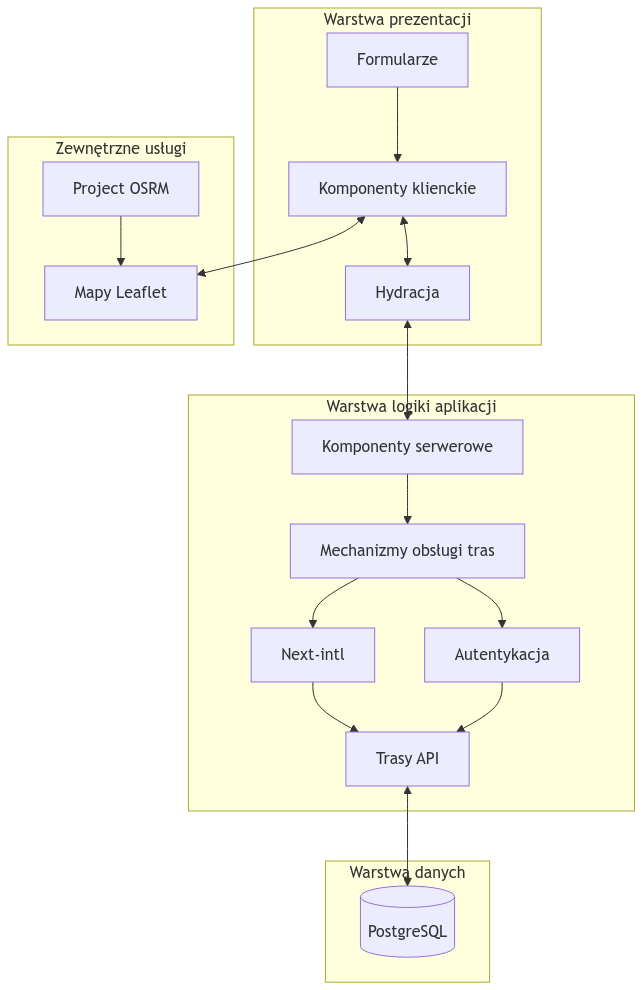
\includegraphics[width=0.7\linewidth]{rozdzial2/diagram_warstw.png}
	\caption{Diagram architektury warstw aplikacji}
	\label{Diagram warstw}
\end{figure}
Powyższy diagram przedstawia architekture warstw aplikacji. Zostały na nim wyszczególnione następujące warstwy:
\begin{enumerate}
    \item \textbf{Warstwa prezentacji} - odpowiada za bezpośrednią interakcje z użytkownikiem. W jej skład wchodzą:
    \begin{enumerate}
        \item formularze - stanowią pośrednika między użytkownikiem, a warstwą logiki aplikacji. Pozwalają na wysyłanie wprowadzonych danych do warstwy logiki aplikacji,
        \item komponenty klienckie (ang. \emph{client components}) - interaktywne elementy interfejsu użytkownika renderowane po stronie przeglądarki końcowego użytkownika, które:
        \begin{itemize}
            \item obsługują zdarzenia użytkownika (kliknięcia, wprowadzanie danych),
            \item zarządzają stanem lokalnym aplikacji przy użyciu \emph{React hooks},
            \item implementują dynamiczne zachowania interfejsu bez przeładowywania strony,
            \item komunikują się z API poprzez żądania HTTP,
            \item renderują interaktywne elementy mapy przy użyciu biblioteki Leaflet.
        \end{itemize}
        \item hydracja - kluczowy proces w architekturze aplikacji \texttt{Next.js}. Przekształca początkowy, statyczny widok strony w pełni interaktywną aplikację React. Poprzez wypełnianie komponentów klienckich danymi pozyskanymi z warstwy logicznej aplikacji.
    \end{enumerate}
    \item \textbf{Warstwa logiki aplikacji} - są w niej zawarte wszelkie mechanizmy, do których użytkownik końcowy nie może mieć wglądu z uwagi na bezpieczeństwo. Warstwa ta składa się z:
    \begin{enumerate}
        \item komponentów serwerowych (ang. \emph{server components}) - komponenty intefejsu użytkownika, które:
        \begin{itemize}
            \item są renderowane po stronie serwera, a użytkownikowi zwracany jest gotowy kod HTML,
            \item redukują ilość JavaScript przesyłanego do przeglądarki,
            \item mogą bezpośrednio komunikować się z bazą danych,
            \item mają dostęp do wrażliwych danych i zmiennych środowiskowych,
            \item są odpowiednie do renderowania statycznej zawartości i elementów niewymagających interaktywności.
        \end{itemize}
        \item mechanizmów obsługi tras (ang. \emph{route handlers}) - odpowiadają za przetwarzanie żądań przychodzących i wysyłanie odpowiedzi.
        \begin{itemize}
            \item obsługują metody HTTP (\emph{GET, POST, PUT, DELETE}),
            \item zapewniają bezpieczną komunikację między frontendem a backendem aplikacji.
        \end{itemize}
        \item Next-intl - biblioteka do internalizacji, jest ona wykorzystywana do prezentacji treści w różnych językach (polskim, angielskim oraz niemieckim).
        \item Autentykacja - zapewnia bezpieczeństwo poprzez blokowanie wybranych tras API nieautoryzowanym użytkownikom.
        \item Trasy API - specjalne endpointy w aplikacji, są wykorzystywane do:
        \begin{itemize}
            \item zarządzania ogłoszeniami (dodawanie, zatwierdzanie, usuwanie zleceń),
            \item obsługi procesu rejestracji i logowania użytkowników,
            \item pobierania i filtrowania listy dostępnych ogłoszeń,
            \item komunikacji z zewnętrznym API OSRM dla wyznaczania tras,
        \end{itemize}
    \end{enumerate}
    \item \textbf{Warstwa danych} - warstwa odpowiadająca za przechowywanie oraz dostarczanie wszelkich danych aplikacji. W aplikacji wykorzystano relacyjną bazę danych PostgreSQL, która przechowuje informacje o:
    \begin{enumerate}
        \item użytkownikach systemu i ich rolach,
        \item zleceniach transportowych i ich statusach,
        \item lokalizacjach geograficznych (punkty początkowe i końcowe tras),
        \item czatach między użytkownikami oraz umowami zawartymi między nimi,
    \end{enumerate}
    \item \textbf{Zewnętrzne usługi} - systemy i API wykorzystywane do rozszerzenia funkcjonalności aplikacji:
    \begin{enumerate}
        \item Project OSRM (ang. \emph{Open Source Routing Machine}), używany jest do zapewnia funkcji wyznaczania tras między punktami. Oferuje API do integracji z aplikacjami transportowymi.
        \item Mapy Leaflet, jest to biblioteka służąca do interaktywnej wizualizacji map, która umożliwia wyświetlanie markerów lokalizacji. Pozwala również na rysowanie tras na mapie oraz zapewnia intuicyjną nawigację i przybliżanie mapy.
    \end{enumerate}
\end{enumerate}
